\documentclass{ruthesis}
\usepackage{graphicx}          % Include this line if your
                               % document contains figures,
%\usepackage[dvips]{epsfig}    % or this line, depending on which
                               % you prefer.
\usepackage{amsfonts,amssymb,amsbsy}
\usepackage{latexsym}
\usepackage{amsmath}
\usepackage{color}
\usepackage{graphics} % for pdf, bitmapped graphics files
\usepackage{epsfig} % for postscript graphics files
\usepackage{epstopdf}
\usepackage{caption}
\usepackage{subcaption}
\usepackage{longtable}
\usepackage{multirow}
\usepackage{afterpage}
\usepackage{array,booktabs,enumitem}% http://ctan.org/pkg/
\newcolumntype{P}[1]{>{\endgraf\vspace*{-\baselineskip}}p{#1}}
%\usepackage{graphicx,subfigure}
%\usepackage{rotating}
%\usepackage{theorem}
%%\usepackage{isomath}
%\usepackage{mathrsfs}
%\usepackage{enumerate}

\usepackage{placeins}
\usepackage{rotating}
\usepackage{titlesec}
\usepackage{geometry}
 \geometry{
 a4paper,
 total={210mm,297mm}, left=20mm, right=20mm, top=20mm, bottom=20mm,}
 
\def\etal{\mbox{et al.}}
\DeclareMathOperator*{\sign}{sign}
\DeclareMathOperator*{\diag}{diag}
\DeclareMathOperator*{\proj}{proj}
\DeclareMathOperator*{\argmin}{argmin}
\DeclareMathOperator*{\rank}{rank}
\newcommand{\norm}[1]{{{\lVert #1 \rVert}}}
\newcommand{\clN}{{\cal N}}
\newcommand{\clM}{{\cal M}}
%\newcommand{\diag}{{\sf diag}}
%\newcommand{\sgn}{{\sf sgn}}
\newtheorem{proposition}{Proposition}
\newtheorem{theorem}{Theorem}
\newtheorem{lemma}{Lemma}
\newtheorem{corollary}{Corollary}
\newtheorem{remark}{Remark}
\newtheorem{definition}{Definition}
\newtheorem{assumption}{Assumption}

\setlength{\parskip}{0.2cm} 
\setlength{\topmargin}{-0.4cm}
\setlength{\oddsidemargin}{1cm} 
\setlength\evensidemargin{1cm}
\setlength{\textwidth}{15cm} 
\setlength{\textheight}{23.5cm}
\titlespacing\section{-4pt}{12pt plus 4pt minus 2pt}{0pt plus 2pt minus 2pt}
\titlespacing\subsection{0pt}{12pt plus 4pt minus 2pt}{0pt plus 2pt minus 2pt}
\titlespacing\subsubsection{0pt}{12pt plus 4pt minus 2pt}{0pt plus 2pt minus 2pt}
\titleformat{\subsubsection}
  {\bfseries\itshape\normalsize}{\thesubsubsection}{1em}{}

\begin{document}
\tableofcontents

\pagenumbering{arabic}
\linespacing{1.7}

\setcounter{chapter}{3}
\chapter{A data assimilating state-space model for algal growth under controlled conditions within a photobioreactor}\label{ch:Intro}


\section{Introduction}\label{sec:micro_intro} 

Microalgae are tiny organisms.. 









\section{Methods}

\subsection{Data Model: Data description and collection methods}

O$_2$, pH, DIC and alk observations collected over 4 days.


Gas, temperature, light and dilution rate were used as forcings.



\subsection{Process model: Carbon chemistry}

To calculate the carbon chemistry of the photo-bioreactor, we would ideally use CO2SYS \cite{lewis1998program} to calculate HCO$_3^-$, CO$_2$, CO$_3$ and pH. 
CO2SYS is a program developed for CO$_2$ system calculations (CO2SYS) that calculates and returns a detailed state of the carbonate system of oceanographic water samples in seawater and freshwater \cite{lewis1998program}.
It uses two of the four measurable carbonate system parameters (total alkalinity, total inorganic CO$_2$, pH, and either fugacity fCO$_2$ or partial pressure of CO$_2$) to calculate the other two parameters at a set of input conditions (temperature and pressure). 

To incorporate CO2SYS into LiBbi for solving carbon chemistry on the timescale of the microalgae model, we explicitly define 2 iterations of the Newton-Raphson method for finding approximations to roots of real valued functions. The Newton-Raphson method is an iterative process considering a function, its derivative and an initial starting value. Vital to the convergence of the Newton-Raphson method is a good starting value. To provide a good starting value, we randomly sample from a range of CO2SYS input parameters (temperature = 20-30, salinity = 30-40, DIC = 200-2500, and alkalinity = 1500-3000) and fit an approximating equation to pH as a function of DIC, S and T (alk?). This gives us a close initial starting value for the Newton-Raphson method. 

Converges in 2-3 iterations 


%%
%% additional info
%%

Choice of H2CO3 and HCO3- dissociation constants K1 and K2 was Mehrbach (refit BY DICKSON AND MILLERO) [BM: After the iterative approach is finalised, the K1 and K2 constants are adjusted based on measurements taken during the experiment, K1*1.23 and K2*0.53 measured during experiment] temperature: 2-35,  salinity: 20-40, Seawater scale, Artificial seawater.



The CO2SYS Matlab version \cite{van2011matlab} was used to produce values of CO$_2$ and HCO$_3^-$ across DIC range 200-2500. 
Approximating equations were fit


Total inorganic CO$_2$ (TCO$_2$) is the sum of the dissolved CO$_2$, the carbonate (CO$_{3-2}$), and the bicarbonate (HCO$_3^-$).




\subsection{Process model: Gas transfer equilibrium concentrations for O$_2$ and CO$_2$}

%Weiss 1970 (O2) and 1974 (CO2) 

%\begin{equation}
%\begin{aligned}
%ln(Ko) =  A_{1} + A_{2}(100/T) + A_{3} ln(T/100) + S\% [B_{1} + B_{2}(T/100) + %B_{3}(T/100)^2 ] 
%\end{aligned}
%\end{equation}

The equilibrium concentration for CO$_2$ solubility in water CO$_{2H}$ ($\mu$mol/L) is calculated using Henry's law,
\begin{equation}\label{eq:CO2H_eq}
CO_{2H}=K0_{CO2}*fCO2*1.0220*1e6
\end{equation}
where fCO2 (atm) is the fugacity or approximately the partial pressure of CO$_2$, 1.0220 is the density of seawater (kg/L) at salinity 34 ppt and temperature 27$^{\circ}$C \cite{ramsing2011seawater} \cite{greensberg1992standard}. K0$_{CO2}$ (mol/kg$_{soln}$/atm) is the solubility of gas in seawater [BM: ask Chris: solubility of gas? is this right] and is calculated from the fitted van't Hoff equation and the logarithmic Setchenow salinity dependence \cite{weiss1974carbon},
\begin{equation}
\begin{aligned}
K0_{CO2} = exp(- 60.2409 + 93.4517(100/T_K)  + 23.3585*ln(T_K/100)+ \\
S(0.023517 - 0.023656(T_K/100) + 0.0047036(T_K/100)^2))
\end{aligned}
\end{equation}
where T$_K$ is the temperature (K) and S is salinity (ppt).

%% from Weiss 1974 paper:
%K0 may be expressed either in moles/1 * atm, referring to a liter of solution at %the temperature of the measurement and an atmosphere fugacity in
%the gas phase, or in moles/kg * atm, referring to a kilogram of solution.



Similarly the equilibrium concentration for O$_2$ solubility in water O$_{2H}$ is calculated using Henry's law,
\begin{equation}\label{eq:O2H_eq}
O_{2H}=K0_{O2}*fO2*1.0220*1e-6
\end{equation}
where fO2 (atm) is the fugacity or approximately the partial pressure of O$_2$, 1.0220 is the density of seawater (kg/L) at salinity 34 ppt and temperature 27$^{\circ}$C \cite{ramsing2011seawater} \cite{greensberg1992standard}, and K0$_{O2}$ (mol/kg$_{soln}$/atm) is the solubility of oxygen in seawater with an adjusted salinity dependence \cite{battino1983solubility},
\begin{equation}
\begin{aligned}
K0_{O2} =  (exp(-1282.8704 + 36619.96/T_K + 223.1396*log(T_K) -0.354707*T_K \\
+ S*(5.957e-3 -3.7353/T_K) + 3.68e-6*S^2))/0.2094e-6
\end{aligned}
\end{equation}
where T$_K$ is the temperature (K) and S is salinity (ppt).


%from Weiss 1970:
%\begin{equation}
%\begin{aligned}
%K0_{O2} = exp(- 58.3877 + 85.8079(100/T_K)  + 23.8439*ln(T_K/100) + \\
%S(-0.034892 + 0.015568(T_K/100) - 0.0019387(T_K/100)^2))
%\end{aligned}
%\end{equation}

The equilibrium concentrations for O$_2$ and CO$_2$ are modelled together with the gas turning on and off during the experiment, as
\begin{equation}
  kLA_{O2} \xi (O_{2H} - O_{2})
\end{equation}
\begin{equation}
0.893 kLA_{O2} \xi (CO_{2H} - CO_{2})
\end{equation}
where $\xi$ is the gas state (1= on, 0= off), and kLA$_{O2}$ is the mass transfer coefficient for air (d$^{-1}$), and 0.893 is the ratio between measured O$_2$ and CO$_2$ mass transfer constants \cite{grima1993gas}.



\subsection{Process model: Photosynthesis and respiration}

Net photosynthesis
\begin{equation}
dDIC/dt  =  -P_1*I*mm + R_1 
\end{equation}
\begin{equation} 
dO_2/dt	 =  \frac{P_1*I*mm - R_1}{R_Q}
\end{equation}

Photosynthesis (P$_1$) and respiration (R$_1$) are both modelled as random walks, by taking \begin{math}P\end{math} and \begin{math}R\end{math}, previously constant parameters, and replacing them by \begin{math}P_1(t)\end{math} and \begin{math}R_1(t)\end{math}. Here, we take \begin{math}P_1(t)\end{math} and \begin{math}R_1(t)\end{math} to be such that
\begin{displaymath}
P_1(t+\Delta t) = P_1(t) + r_P
\end{displaymath}
\begin{displaymath}
R_1(t+\Delta t) = R_1(t) + r_R
\end{displaymath}
where \begin{math}
r_P \sim N(0, \sigma_{r_P})
\end{math}, \begin{math}
r_R \sim N(0, \sigma_{r_R})
\end{math}, and \begin{math}
\Delta t
\end{math} is the length of discrete time-step. For the purpose of the Bayesian analysis here, \begin{math}\sigma_{r_P}\end{math} and \begin{math}\sigma_{r_R}\end{math} are treated as a parameter to be inferred. 


R$_Q$ is the respiratory quotient, the ratio of CO$_2$ produced and O$_2$ consumed by a cell. 





PAC is Photosynthetically Active Carbon, this is the type of carbon that the microalgae use for photosynthesis. This can be CO$_2$, HCO$_3^-$, or a combination of both, eg $PAC = CO_2 + HCO_3^-$ if the microalgae are using both carbon dioxide and bicarbonate for photosynthesis.  

\begin{equation}
PAC = HCO_3^-
\end{equation}


\begin{equation}
mm = \frac{PAC}{K_m + PAC} 
\end{equation}

\subsection{Process model: Ordinary differential equations}

Ode's:
%\begin{equation}
\begin{align}
\text{Rate} & & \text{flux into cells}            &            &\text{gas transfer}   &     & \text{dilution} \nonumber                              \\
\frac{\partial DIC}{\partial t}&=&                      - (P - R)&      &+\hat Q^{air}kLa_{ CO_2}^{air}(CO_{2}^{air} - CO_{2})                  & &+\frac{Q^M}{V}(DIC^{M} - DIC)       \nonumber \\
                                           &  &                                   &      &+\hat Q^{co2}kLa_{ CO_2}^{co2}(CO_{2}^{co2} - CO_{2})    \\
\frac{\partial O_2}{\partial t}&=& \frac{1}{R_Q}  (P - R)&      &+\hat Q^{air}kLa_{\phantom{C}O_2}^{air}(\phantom{C}O_{2}^{air} -   \phantom{CC}O_{2}) && +\frac{Q^M}{V}(\phantom{C}O_{2}^{M} - \phantom{CC}O_{2})     \nonumber   \\
                                           &  &                                   &      &+\hat Q^{co2}kLa_{\phantom{C}O_2}^{co2}(\phantom{C}O_{2}^{co2} - \phantom{C}O_{2})    \\
\frac{\partial TA}{\partial t} & =&      R_R (P \phantom{ + R})& & & & +\frac{Q^M}{V}(\phantom{C}TA^{M} - \phantom{C}TA)
\end{align}
%\end{equation}


%\begin{table}[ht]
%\caption{Multi-row table}
%\begin{center}
%\begin{tabular}{|c|c|c|c|c|}
\begin{longtable}{|c|c|c|c|c|}
	\hline 
	& Symbol & Description  & Prior / Value & Unit \\
    \hline
    \multirow{4}{*}{\rotatebox[origin=c]{90}{State variable initial conditions }}
    & $DIC^0$ & Dissolved inorganic carbon &  & $\mu$M/L \\
    & $O_2^0$ & Oxygen &  & $\mu$M/L \\
    & TA$^0$  & Total alkalinity & & $\mu$M/L \\
    & P$^0$  & Rate of photosynthesis & & $\mu$M/L/day\\
    & R$^0$  & Rate of respiration & & $\mu$M/L/day\\
    & pH$^0$ & -  & & log$_{10}$(-mol/L H+)  \\
    & $CO_2$$^0$ & Carbon dioxide  & & $\mu$M/L \\
    & $HCO_3^-$$^0$ & Bicarbonate & & $\mu$M/L  \\
    & $CO_3^{2-}$$^0$ & Carbonate &  & $\mu$M/L \\
    \hline
    \multirow{4}{*}{\rotatebox[origin=c]{90}{Gas transfer terms }}
    &$ \hat Q ^{air} $ &indicator for flow in air line  & 0 or 1 & - \\
    & $x_{CO_2}^{air} $ & mole fraction of CO$_2$ atmosphere& 400 & ppm \\ 
    & $CO_{2H}$  & Equilibrium CO$_2$ concentration  & Eq. \ref{eq:CO2H_eq} & $\mu$M/L  \\
    & $CO_{2}^{air}$ & sat CO$_2$ conc with atmosphere &   $x_{CO_2}^{air} CO_{2H}$ & \\
    & $kLa_{ CO_2}^{air}$ & Mass transfer coefficient for CO$_2$ & 0.893$kLa_{\phantom{C}O_2}^{air}$  & day$^{-1}$ \\
    
    & $x_{O_2}^{air} $ & mole fraction of O$_2$ atmosphere& 0.2094 & atm \\ 
    & $\phantom{C}O_{2H}$  & Equilibrium O$_2$ concentration  & Eq. \ref{eq:O2H_eq} & $\mu$M/L  \\
	& $\phantom{C}O_{2}^{air}$ & sat O$_2$ conc with atmosphere &   $x_{O_2}^{air} O_{2H}$ & \\
    & $\tau$ & half-life of $kLa_{\phantom{C}O_2}^{air}$  & range(2-20) & min$^{-1}$\\
    & $kLa_{\phantom{C}O_2}^{air}$ & Mass transfer coefficient for O$_2$ & $\ln(2) * 24*60/\tau$ & day$^{-1}$\\
   
    \hline
        \multirow{4}{*}{\rotatebox[origin=c]{90}{Dilution terms }}
    &$  Q ^{M} $ & rate  &  & ml/day \\
    &$  V $ & Volume of the reactor  & 500 & ml \\
    &$  DIC ^{M} $ & Media dissolved inorganic carbon  & 1724.20 & $\mu$M/L \\ 
    &$	\phantom{CC}O_2^{M}$ & Media oxygen concentration & 226.65 & $\mu$M/L \\
    &$	\phantom{C}TA^{M}$  & Media total alkalinity & 1797.90 & $\mu$M/L
    \\
    
        \hline
    \multirow{4}{*}{\rotatebox[origin=c]{90}{Other dilution terms }}
    &$ \hat Q ^{CO2} $ &indicator for dilution & 0 or 1 & - \\
  
    & $x_{\phantom{C}O_2}^{CO2} $ & mole fraction of & 0 & - \\ 
    & $\phantom{C}O_{2}^{CO2}$ & sat CO$_2$ conc with CO$_2$ &   $x_{O_2}^{CO2} O_{2H}$ & \\
    & $kLa_{ \phantom{C}O_2}^{CO2}$ & mass transfer coefficient &   & day$^{-1}$ \\
    & $\phantom{C}O_2^{CO2}$  & & & \\
    
    & $x_{CO_2}^{CO2} $ & mole fraction of  & 1 & ppm \\ 
    & $CO_{2}^{CO2}$ & sat CO$_2$ conc with CO$_2$ &   $x_{CO_2}^{CO2} CO_{2H}$ & \\
    & $kLa_{ CO_2}^{CO2}$ & mass transfer coefficient & 0.893$kLa_{\phantom{C}O_2}^{CO2}$  & day$^{-1}$ \\
    &$  CO_{2} ^{CO2} $ &   &  &  \\   
    \hline
\end{longtable}  
    
%\end{tabular}
%\end{center}
%\label{tab:multicol}
%\end{table}


\clearpage
\begin{tabular}{l l  | l}
	 \hline 
	Symbol & Variable & Units  \\ \hline
	DIC &  Dissolved inorganic carbon concentration & $\mu$mol/L  \\
	O$_2$ & Oxygen  &  $\mu$mol/L \\
%	B & Microalgae population & concentration of cells**[BM]  \\
	pH & -  & log$_{10}$(-mol/L H+)  \\
	CO$_2$ & Carbon dioxide  & $\mu$mol/L \\
	HCO$_3^-$ & Bicarbonate & $\mu$mol/L  \\
	CO$_3^{2-}$ & Carbonate  & $\mu$mol/L \\
	PAC & Photosynthetically active carbon & $\mu$mols/L  \\
	mm & - & - \\
	kLA$_{O2}$  & Mass transfer coefficient for O$_2$ &  d$^{-1}$  \\
	
	CO$_{2H}$  & Equilibrium CO$_2$ concentration  & $\mu$mols/L  \\
	
	K0$_{O2}$ &  Solubility of gas & mol/kg$_{soln}$/atm  \\
	K0$_{CO2}$ & Solubility of gas & mol/kg$_{soln}$/atm   \\
	TA  & Total alkalinity & $\mu$mols/L  \\
	S  & Salinity &  ppt  \\
	fCO2  & Fugacity/CO$_2$ partial pressure &  atm  \\
	fO2  & Fugacity/O$_2$ partial pressure &  atm \\
	
	K$_m$ & Carbon restriction & $\mu$mols/L \\
	
	P & Photosynthesis rate & $\mu$mols/L/day \\
	R & Respiration rate & $\mu$mols/L/day \\
	R$_R$ & Redfield ratio & - \\	
	R$_Q$ & Respiratory quotient & - \\
\end{tabular}
\captionof{table}{Table of variables and parameters.}

\begin{tabular}{c c  | c}
	 \hline
	 Symbol & Variable & Units  \\ \hline
	I &  Light Intensity  &  normalised to 0-1   \\
	T & Temperature & $\circ$ C  \\
	T$_K$ & Temperature &  K  \\
	$\xi$ & gasflow &  on/off (1,0)  \\
	
\end{tabular}
\captionof{table}{Table of Forcings}


\subsection{Parameter Model: Priors}
Decide whether the parameters vary in time or not.




\begin{tabular}{c | c  |  c}
	Parameter & Prior &  Proposal \\ \hline
	S  & 34 & * \\
	fCO2  & 397e-6 &  *  \\
	fO2  & 0.21 &  *  \\
	kLA$_{O2}$  & LogNormal(log(200.0), 0.5)  & LogNormal(log(kLA$_{O2}$), 0.5prop$_{std}$) \\
	K$_m$ &  LogNormal(log(200.0), 0.8)  & LogNormal(log(K$_m$), 0.8prop$_{std}$) \\
	R$_R$  & Uniform(0.0001, 0.2) &  TrunNormal(R$_R$, 0.2prop$_{std}$, 0.0001, 0.2) \\
	R$_Q$  & Uniform(0.66, 1) &  TrunNormal(R$_Q$, 0.2prop$_{std}$, 0.66, 1.0)
	 \\
	$\sigma_P$ & Normal(0.05, 0.01) & Normal($\sigma_P$, 0.01prop$_{std}$) \\
	$\sigma_R$ & Normal(0.01, 0.001) & Normal($\sigma_R$, 0.001prop$_{std}$) \\
	
%R$_1$ & LogNormal(log(1000.0), 0.3)  & LogNormal(log(R$_1$), 0.3prop$_{std}$) \\	
%	P$_1$ & 4.7407e-4 $\pm$ & - \\
\end{tabular}
\captionof{table}{Table of Parameters, their priors and proposal distributions. * indicates the parameter was held fixed. (prop$_{std}$ =0.1)}
\newpage


\FloatBarrier

\section{Results}


\subsection{Carbon chemistry iterative solution}

Total Sulfur
\begin{align*}
 TS     	&= \frac{0.14}{96.062}*\frac{S}{1.8065} \nonumber \\
 IS     	&= 19.924*\frac{S}{(1000.0 - 1.005*S)} \nonumber \\
 KS_{int} 	&= -\frac{4276.1}{T_K} + 141.328 - 23.093*log(T_K) + (-\frac{13856.0}{T_K} + 324.57 \nonumber\\ 			 
 			& - 47.986*log(T_K))*\sqrt{IS} + ( \frac{35474}{T_K} - 771.54  + 114.723*log(T_K))*IS \nonumber \\
 			& - \frac{2698}{T_K}*IS^{1.5} + \frac{1776}{T_K}*IS^2 \nonumber \\
 KS     	&= exp(KS_{int})*(1 - 0.001005*S) \nonumber \\
\end{align*}

Fluorine
\begin{align*}
TF       	&= 0.000067*S/18.9984/1.80655 \nonumber \\
KF       	&= exp(-(-\frac{874.0}{T_K} - 0.111*\sqrt{S} + 9.68)) \nonumber \\
SWS_{2_T}  	&= \frac{(1 + \frac{TS}{KS})}{(1 + \frac{TS}{KS} + \frac{TF}{KF})} \nonumber \\
Free_{2_T} 	&= 1 + \frac{TS}{KS} \nonumber \\
\end{align*}


\begin{align*}
\text{H2O dissoc} \nonumber \\
KW 		&= exp(148.9802 - \frac{13847.26}{T_K}  - 23.6521*log(T_K) \nonumber \\
		&+ (\frac{118.67}{T_K} - 5.977 + 1.0495*log(T_K))*\sqrt{S} - 0.01615*S) \nonumber \\
\text{Boron} \nonumber \\
KB 		&= exp((-8966.90 - 2890.53*\sqrt{S} - 77.942*S \nonumber \\
		&+ 1.728*S*\sqrt{S} - 0.0996*S^2)/T_K + 148.0248 \nonumber \\
		& + 137.1942*\sqrt{S} + 1.62142*S \nonumber \\
		&- (24.4344 + 25.085*\sqrt{S} + 0.2474*S)*log(T_K)  \nonumber \\ 
		&+ 0.053105*\sqrt{S}*T_K) \nonumber \\
TB 		&= 0.0004326*\frac{S}{35} \nonumber \\
\text{Carbon eq constants} \nonumber \\
K1 		&= 10^{(-(\frac{3633.86}{T_K} - 61.2172 + 9.6777 *log(T_K) - 0.011555*S + 0.0001152*S^2))}*1.23	\nonumber \\
K2 		&= 10^{(-(\frac{471.8}{T_K} + 25.9290 - 3.16967*log(T_K) - 0.01781*S + 0.0001122*S^2))}*0.53 \nonumber \\	
\end{align*}
1.23 and 0.53 were experiment specific and measured 


Initial guess at the pH 
\begin{align*}
pH_{init} 	&= 12.26 -0.0030605*DIC -0.043752*T -0.013625*S+ 0.00011315*TA \nonumber \\
&+ 1.3463e-5*DIC*T + 5.2215e-7*DIC*TA \nonumber \\
\end{align*}

Iterations
\begin{align*}
h 			&=  10^{-pH_{init}}	\nonumber                              \\
h_{free} 	&=  \frac{h}{Free_{2_T}}	 \nonumber \\
f0 			&= (  DIC*1e-6*\frac{K1*h+2*K1*K2}{h*h+K1*h+K1*K2}    \nonumber\\
			&  - h_{free} + \frac{KW}{h} - Alk*1e-6 + \frac{TB}{1+\frac{h}{KB}} )*1e6 \nonumber  \\
df0 		&= (  DIC*1e-6*\frac{K1 +2*K1*K2}{h^2+K1*h+K1*K2}  \nonumber\\
			&  -DIC*1e-6*\frac{(K1*h+2*K1*K2)}{(h^2+K1*h+K1*K2)^2}*(2*h+K1)  \nonumber\\
			&  -TB *\frac{1}{(1+ \frac{h}{KB})^2} / KB             \nonumber             \\
			&  -\frac{KW}{h^2} - \frac{1}{Free_{2_T}} )*1e6  * (-log(10)*10^{-pH}) \nonumber \\
pH 			&= pH - \frac{f0}{df0} \nonumber                              \\
H 			&= 10^{-pH} \nonumber                              \\
denom 		&= H^2+K1*H+K1*K2 \nonumber                              \\
CO2  		&= \frac{DIC*H^2}{denom} \nonumber                              \\
HCO3 		&= \frac{DIC*H *K1}{denom} \nonumber                              \\
CO3  		&= \frac{DIC*K1*K2}{denom}      \nonumber \\                         
\end{align*}




\begin{figure}
	\centerline{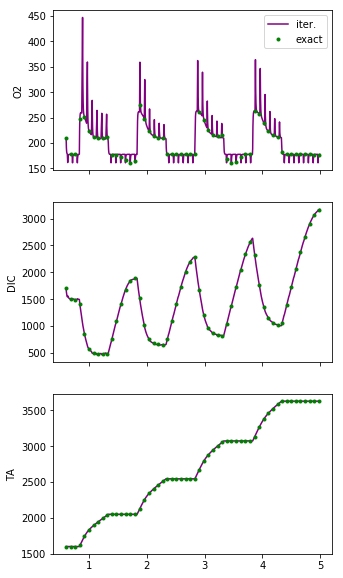
\includegraphics[width=0.5\textwidth]{images_microalgae/plots/iterative_states}}
	\caption[.]{Field study}
	\label{fig:iterative_states}
\end{figure}


\begin{figure}
	\centerline{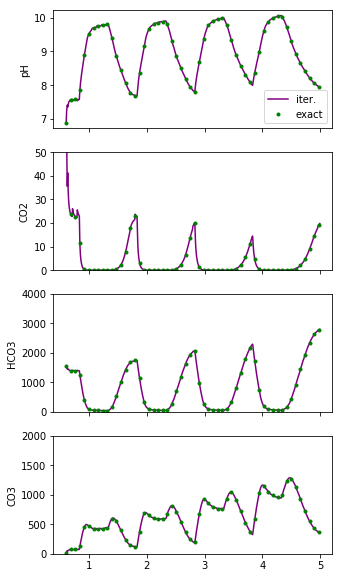
\includegraphics[width=0.5\textwidth]{images_microalgae/plots/iterative_carbon}}
	\caption[.]{Field study}
	\label{fig:iterative_carbon}
\end{figure}

\begin{table}
\begin{tabular}{|c|c|c|c| c | c|} 
\hline
\bfseries{Variable} & \bfseries{Iter. 1} & \bfseries{Iter. 2} & \bfseries{Iter. 3}  &  \bfseries{Iter. 4} & \bfseries{Iter. 5} \\ \hline
$O_2$		&  0.308389964	&0.016044284	&4.18E-05		&6.89E-05		&7.59E-05 		\\
$DIC$		& 16.78775711	&0.958511825	&0.005229318	&0.002305054	&0.002333411 	\\
$TA$		&  2.607767674	&0.160897272	&0.000688102	&0.001257725	&0.001218981 	\\
$pH$		& 0.036092734	&0.002355758	&1.41E-05		&6.93E-06		&6.93E-06 		\\
$CO2$		& 2.109401968	&0.145719349	&0.001222812	&0.000866728	&0.000866727 	\\
$HCO3$		& 19.81869214	&1.21021115		&0.008016765	&0.001025002	&0.001025139 	\\
$CO3$		& 20.89660704	&1.307061652	&0.00867642		&0.001102278	&0.001102434 	\\
\hline
\end{tabular}
\caption{RMSE for 5 iterations of the Newton-raphson carbon chemistry iterative solution.}
\label{table:rmse_iterative}
\end{table}


%Approximating equations in place of CO2SYS:
%
%\begin{equation}
%\begin{aligned}
%HCO_3^- = exp(16.262 + 0.0047081*DIC - 0.11922*T + 0.0050303*alk1 \\
%+ 1.7093*log(DIC) + 0.38048*log(S) - 3.7548*log(alk1)\\
%- 2.292e-5*DIC*T - 0.0032028*DIC*log(DIC) - 0.00015313*DIC*log(S)\\
%+ 0.0032527*DIC*log(alk1) +\\ 0.021965*T*log(alk1) - 0.00090344*alk1*log(DIC))
%\end{aligned}
%\end{equation}
%
%\begin{equation}
%\begin{aligned}
%CO_2 = exp(-486.84 - 0.070754*DIC - 0.25277*T - 0.20674*S - \\
%0.11627*alk1 + 78.274*log(DIC) + 72.147*log(alk1) - 2.9438e-5*DIC*T\\
% - 5.8841e-6*DIC*alk1 - 0.0040234*DIC*log(DIC) + 0.016172*DIC*log(alk1)\\
% - 0.02039*T*log(DIC) + 0.062452*T*log(alk1) + 0.029857*S*log(alk1) \\
% + 0.0031507*alk1*log(DIC) + 0.010398*alk1*log(alk1) \\
% - 11.192*log(DIC)*log(alk1))
%\end{aligned}
%\end{equation}
%
%\begin{equation}
%\begin{aligned}
%pH = 9.5803 - 0.0027089*DIC - 0.018089*T - 0.012068*S + 0.0016329*alk1\\
%+ 1.2706e-5*DIC*T + 4.6961e-7*DIC*alk1 - 9.2122e-6*T*alk1 - \\
%5.9777e-8*DIC**2 - 2.194e-7*alk1**2 
%\end{aligned}
%\end{equation}



%% For reference

%\begin{equation}
%HCO_3^- =  -818.0204 +   1.9388 DIC  +  0.0681alk  -0.0003 DIC alk
%\end{equation}
%
%\begin{equation}
%\begin{aligned}
%CO_2 = exp(-10.6788 +   0.0096 DIC +   0.1479 T +   0.0330 S  -0.0015 alk \\
%-6.2777e-05 DIC T   - 8.778e-07 DIC alk)
%\end{aligned}
%\end{equation}
%
%\begin{equation}
%\begin{aligned}
%pH = 12.26 -0.0030605 DIC -0.043752 T -0.013625 S+ 0.00011315 alk\\
%+ 1.3463e-05 DIC T + 5.2215e-07 DIC alk
%\end{aligned}
%\end{equation}

\FloatBarrier
\subsection{Posteriors}




%\section{Unscented Kalman Filter}
%
%
%\subsection{Introduction to the Unscented Kalman Filter}
%
%history, how it emerged, when to use it, comparison with other techniques, fast and computationally cheap 
%
%\subsection{Unscented Kalman Filter Algorithm}
%
%\begin{enumerate}
%\item Choose the sigma parameters $\alpha$, $\beta$ and $\kappa$
%\item Define P the covariance estimate matrix, R the measurement noise matrix, and Q the process noise matrix
%\item Find the weights, means and sigma points
%\item Predict step
%\item Update step
%\end{enumerate}
%
%If you already have your whole dataset then you can employ batch processing instead.



\appendix

\chapter{LiBbi model code}\label{appendix_micro_libbi_code}

\textbf{Model file: micro\_iterative.bi}
\begin{verbatim}
/*
* Microalgae model. 
* ode solver every minute, obs and input files are in days
* iterative solution using newton raphson for the CO2SYS solutions
*/
model micro_iterative {

const FO2  = 0.2094
const FCO2 = 397e-6
const S    = 34

param kLAO2
param Km
param RR
param RQ

input I			// light intensity
input T			//temperature (C)
input gas		//gas on/off

state DIC // state variables
state O_2
state pH
state O2H_pr
state CO2H_pr
state R
state R1
state P
state P1
state alk
state CO2
state HCO3
state CO3
state O_2H
state CO2H

noise r_R
noise r_P

/* random walk parameter */
param sigma_r_R
param sigma_r_P

obs O2_obs
obs pH_obs
obs DIC_obs
obs alk_obs

sub parameter {/* prior distribution over parameters */
Km 	~ log_normal(log(200.0), 0.8)
kLAO2 	~ log_normal(log(200.0), 0.5)
RR 	~ uniform(0.0001, 0.2)
RQ	~ uniform(0.66, 1.0)

sigma_r_R 	~ normal(0.01, 0.001)
sigma_r_P 	~ normal(0.05, 0.01)
}


const prop_std = 0.1;
sub proposal_parameter {
Km 	~ log_normal(log(Km), 0.8*prop_std)
kLAO2 	~ log_normal(log(kLAO2), 0.5*prop_std)
RR 	~ truncated_normal(RR, 0.2*prop_std, lower = 0.0001, upper = 0.2)
RQ 	~ truncated_normal(RQ, 0.2*prop_std, lower = 0.66, upper = 1.0)

sigma_r_R 	~ normal(sigma_r_R, 0.001*prop_std)
sigma_r_P 	~ normal(sigma_r_P, 0.01*prop_std)
}

sub initial {/* prior distribution over initial conditions, given parameters */
// specify the initial condition model 
R 	~ normal(log(500.0), 0.6)
R1 	~ log_normal(log(500.0), 0.6)
P 	~ normal(log(5000.0), 0.8)
P1 	~ log_normal(log(5000.0), 0.8)
alk 	~ log_normal(log(1700.0), 0.1)

DIC 	~ log_normal(log(1200.0), 0.2) 
O_2 	~ log_normal(log(230.0), 0.2)   
pH 	~ log_normal(log(8.5), 0.2)
CO2 	~ log_normal(log(3.0), 0.4)
HCO3 	~ log_normal(log(1000.0), 0.3)
CO3 	~ log_normal(log(300.0), 0.4)
O_2H 	~ log_normal(log(200.0), 0.2)	
CO2H 	~ log_normal(log(10.0), 0.2)
}



sub transition(delta = 0.0023) { // obs are in days ie delta=1.0 for daily solving. delta=0.00069 for solving every minute, delta=0.000011574 for solving every second



/* processes */

inline TK     = T + 273.0		// temp in kelvin
inline K0_CO2 = exp(-60.2409 + 93.4517*(100.0/TK) + 23.3585*log(TK/100.0)+ S*(0.023517 - 0.023656*(TK/100) + 0.0047036*(TK/100.0)*(TK/100.0)))
CO2H          <- K0_CO2*FCO2*1.0220*1e6

inline K0_O2  =  (exp(-1282.8704 + 36619.96/TK + 223.1396*log(TK) -0.354707*TK + S*(5.957e-3 -3.7353/TK) + 3.68e-6*S*S))/(0.2094e-06)
O_2H 	      <- K0_O2*FO2*1.0220*1e-6

inline PAC    = HCO3  		//PAC=photosynthetically active carbon. if the phyto are just using CO2 to photosynthesise then PAC=CO2
inline mm     = PAC/(Km+PAC)

// CO2SYS iterative solution
// set up all the constants

inline logTK  = log(TK)
inline S2     = S*S
inline sqrtS  = sqrt(S)

// total sulphur

inline TS     = (0.14/96.062)*(S/1.80655)
inline IS     = 19.924*S/(1000.0 - 1.005*S)

inline KS_int = -4276.1/TK + 141.328 - 23.093*logTK + (-13856.0/TK + 324.57  -  47.986*logTK)*sqrt(IS) + ( 35474.0/TK - 771.54  + 114.723*logTK)*IS - 2698.0/TK*IS**1.5 + 1776.0/TK*IS**2
inline KS     = exp(KS_int)*(1 - 0.001005*S)

// Fluorine

inline TF       = 0.000067*S/18.9984/1.80655
inline KF       = exp(-(-874.0/TK - 0.111*sqrtS + 9.68))
inline SWS_2_T  = (1.0 + TS/KS)/(1.0 + TS/KS + TF/KF)
inline Free_2_T = 1.0 + TS/KS

// H2O dissoc

inline KW = exp(148.9802 - 13847.26/TK  - 23.6521*logTK + (118.67/TK - 5.977 + 1.0495*logTK)*sqrtS - 0.01615*S)

// Boron

inline KB = exp((-8966.90 - 2890.53*sqrtS - 77.942*S + 1.728*S*sqrtS - 0.0996*S2)/TK + 148.0248 + 137.1942*sqrtS + 1.62142*S - (24.4344 + 25.085*sqrtS + 0.2474*S)*logTK + 0.053105*sqrtS*TK)
inline TB = 0.0004326*S/35.0

// Carbon eq constants

inline K1 = 10**(-(3633.86/TK - 61.2172 + 9.6777 *logTK - 0.011555*S + 0.0001152*S**2))
inline K2 = 10**(-( 471.8/TK + 25.9290 - 3.16967*logTK - 0.01781*S + 0.0001122*S**2))

// end all the constants

// intial guess at the pH (use the approximating equation)

//	inline pH_init = 9.5803 - 0.0027089*DIC - 0.018089*T - 0.012068*S + 0.0016329*alk + 1.2706e-05*DIC*T + 4.6961e-07*DIC*alk - 9.2122e-06*T*alk - 5.9777e-08*DIC**2 - 2.194e-07*alk**2 
inline pH_init = 12.26 -0.0030605*DIC -0.043752*T -0.013625*S+ 0.00011315*alk + 1.3463e-05*DIC*T + 5.2215e-07*DIC*alk

// iteration 1

inline h_1 	= 10.0**(-pH_init)
inline h_free_1	= h_1/Free_2_T
inline f0_1 	= (DIC*1e-6*(K1*h_1 + 2.0*K1*K2)/(h_1*h_1 + K1*h_1 + K1*K2) - h_free_1 + KW/h_1 - alk*1e-6 + TB/(1.0 + h_1/KB))*1e6
inline df0_1 	= (DIC*1e-6*(K1 + 2.0*K1*K2)/(h_1**2.0 + K1*h_1 + K1*K2) - DIC*1e-6*(K1*h_1 + 2.0*K1*K2)/(h_1**2.0 + K1*h_1 + K1*K2)**2.0*(2.0*h_1 + K1) - TB*1.0/(1.0 + h_1/KB)**2.0/KB - KW/h_1**2.0 - 1.0/Free_2_T)*1e6*(-log(10.0)*10.0**(-pH_init))
inline pH_1	= pH_init - f0_1/df0_1

// iteration 2

inline h 	= 10.0**(-pH_1)
inline h_free 	= h/Free_2_T
inline f0 	= (DIC*1e-6*(K1*h + 2.0*K1*K2)/(h*h + K1*h + K1*K2) - h_free + KW/h - alk*1e-6 + TB/(1.0 + h/KB))*1e6
inline df0 	= (DIC*1e-6*(K1 + 2.0*K1*K2)/(h**2.0 + K1*h + K1*K2) - DIC*1e-6*(K1*h + 2.0*K1*K2)/(h**2.0 + K1*h + K1*K2)**2.0*(2.0*h + K1) - TB*1.0/(1.0 + h/KB)**2.0/KB - KW/h**2.0 - 1.0/Free_2_T)*1e6*(-log(10.0)*10.0**(-pH_1))
pH 		<- pH_1 - f0/df0    

// calculate the final concentrations

inline H 	= 10.0**(-pH)
inline H2 	= H*H
inline denom 	= (H2 + K1*H + K1*K2)
CO2  		<- DIC*H2/denom
HCO3 		<- DIC*H*K1/denom
CO3  		<- DIC*K1*K2/denom  

// end CO2SYS iterative solution


/* R and P as random walks */

r_R 	~ normal(0.0, sigma_r_R)
R 	<- R + r_R
R1 	<- exp(R)

r_P ~ normal(0.0, sigma_r_P)
P 	<- P + r_P
P1 	<- exp(P)

ode(h = 0.1, atoler = 1.0e-6, rtoler = 1.0e-6, alg = 'RK4(3)'){
dDIC/dt  =  -P1*I*mm + R1 	+ gas*0.893*kLAO2*(CO2H - CO2)  		// DIC = Dissolved Inorganic Carbon 
dO_2/dt	 =  (P1*I*mm - R1)/RQ 	+ gas*kLAO2*(O_2H - O_2)	 		// O_2 = Dissolved Oxygen 
dalk/dt  =   RR*P1*I*mm
}

}


sub observation {

O2_obs  ~ log_normal(log(O_2), 0.3)
pH_obs  ~ log_normal(log(pH), 0.3)
DIC_obs ~ log_normal(log(DIC), 0.3) 
alk_obs ~ log_normal(log(alk), 0.3)
}
}
\end{verbatim}

\textbf{Prior sampling file: prior.conf}
\begin{verbatim}
--target prior
--model-file micro_iterative.bi
--nsamples 500
--start-time 0.61304
--end-time 4.7866
--noutputs 6049
--input-file data/input_all_2018_normalised.nc
--output-file results/prior_micro_iterative.nc
\end{verbatim}

\textbf{Posterior sampling file: posterior.conf}
\begin{verbatim}
--target posterior
--model-file micro_iterative.bi
--input-file data/input_all_2018_normalised.nc
--obs-file data/obs_all_2018.nc
--nsamples 500
--nparticles 1024
--start-time 0.61304
--end-time 4.7866
--noutputs 6049
--output-file results/posterior_micro_iterative.nc
--with-transform-initial-to-param
\end{verbatim}

\begin{sidewaysfigure}
	\centerline{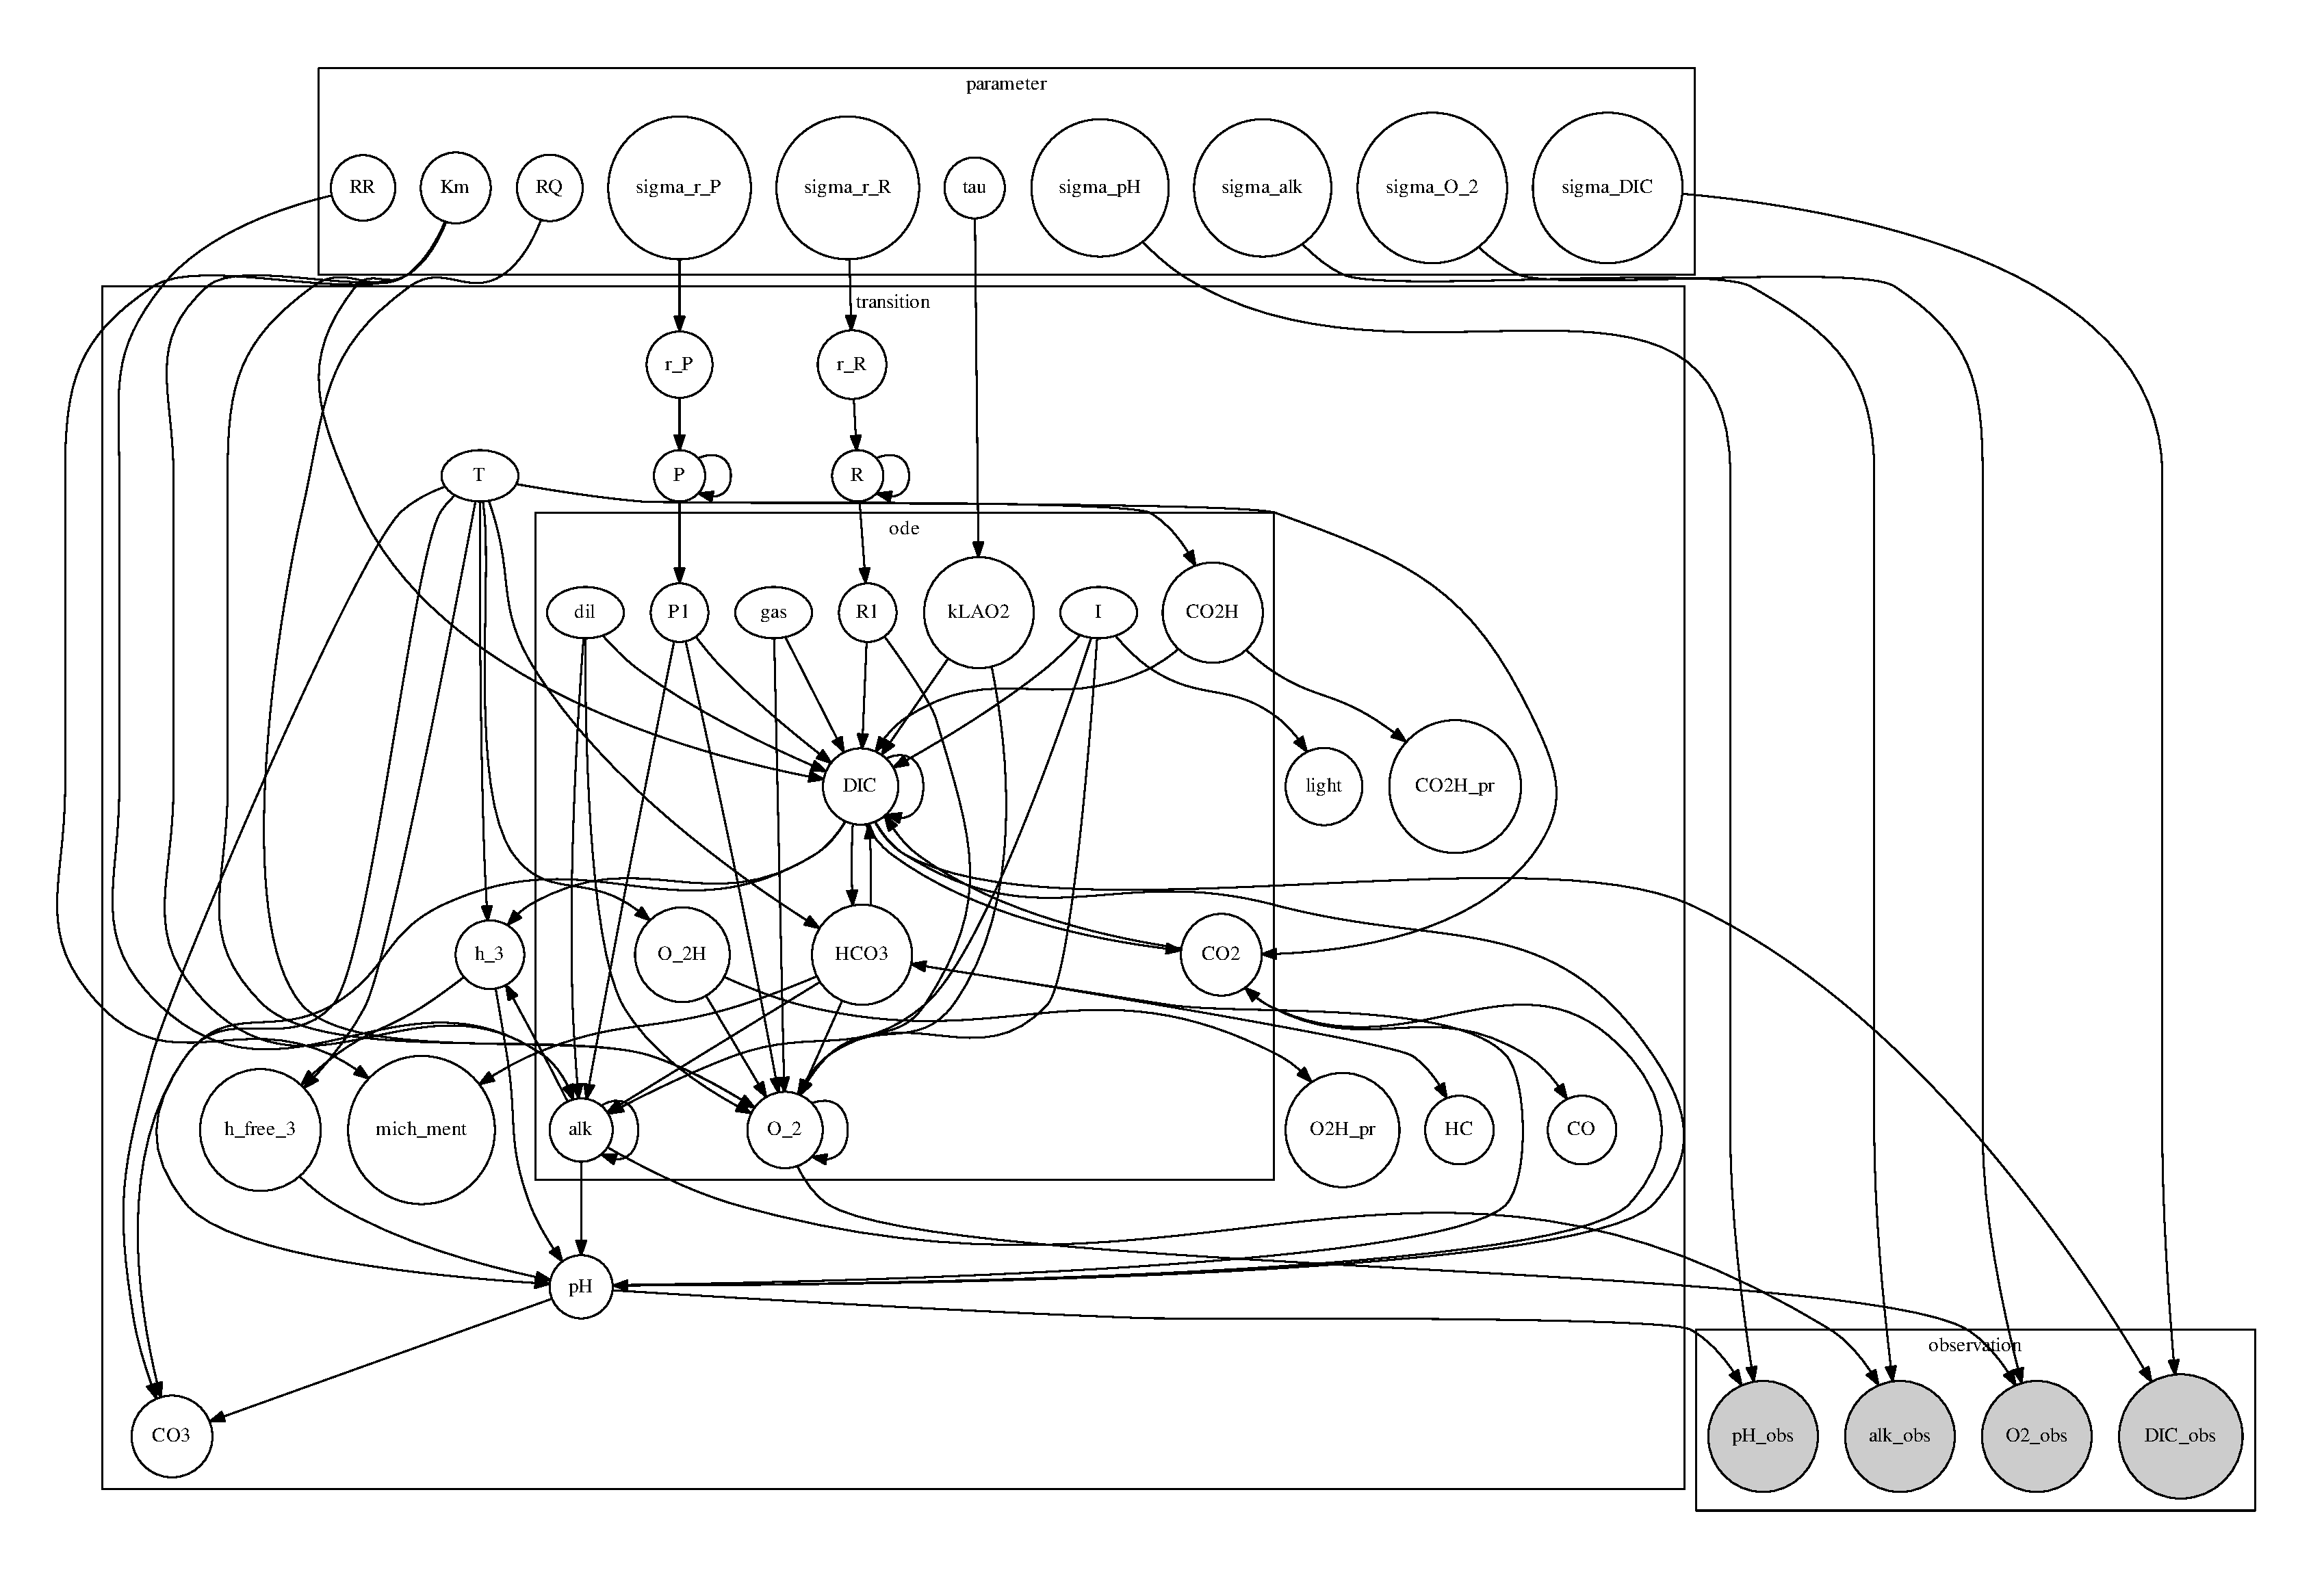
\includegraphics[width=0.9\textwidth]{images_microalgae/micro_template.pdf}}
	\caption[.]{Directed Acyclic Graph of the LiBbi model file micro.bi}
	\label{fig:micro_DAG}
\end{sidewaysfigure}


\bibliography{seagrassbib}{}
\bibliographystyle{plain}

%\ifx\printbibliography\undefined
%\bibliographystyle{plain}
%\bibliography{bibexport}
%\else\printbibliography\fi



\end{document}

